% questions.tex —— 2009 年·全国大纲卷Ⅱ·理科 · 题目内容片段（无答案）
% 由 tools/generate_projects.py 依来源总账自 2009/2009_数学真题_全国2理_试题.md 生成，勿手改（改源 MD 后重跑）


\gkpart{数学}

\begin{gktip}
\textbf{来源说明}：本题面依据固定源 PDF 两页 A3 题面逐题转录，原卷印刷页码 511–512。固定源不附答案，答案和解析均由本库独立复算。

\textbf{图形说明}：第 12、18 题的原卷图形关系重绘为 TikZ/PGFPlots 矢量图。图形标记所指的 PNG 不随仓库保存。
\end{gktip}

\gkpart{一、选择题}

\begin{question}
\gkti{1}$\dfrac{10i}{2-i}=$\mbox{（　　）}

（A）$-2+4i$\quad（B）$-2-4i$\quad（C）$2+4i$\quad（D）$2-4i$

\end{question}
\begin{question}
\gkti{2}设集合 $A=\{x\mid x>3\}$，$B=\left\{x\mid\dfrac{x-1}{x-4}<0\right\}$，则 $A\cap B=$\mbox{（　　）}

（A）$\varnothing$\quad（B）$(3,4)$\quad（C）$(-2,1)$\quad（D）$(4,+\infty)$

\end{question}
\begin{question}
\gkti{3}已知 $\triangle ABC$ 中，$\cot A=-\dfrac{12}{5}$，则 $\cos A=$\mbox{（　　）}

（A）$\dfrac{12}{13}$\quad（B）$\dfrac5{13}$\quad（C）$-\dfrac5{13}$\quad（D）$-\dfrac{12}{13}$

\end{question}
\begin{question}
\gkti{4}曲线 $y=\dfrac{x}{2x-1}$ 在点 $(1,1)$ 处的切线方程为\mbox{（　　）}

（A）$x-y-2=0$\quad（B）$x+y-2=0$\quad（C）$x+4y-5=0$\quad（D）$x-4y-5=0$

\end{question}
\begin{question}
\gkti{5}已知正四棱柱 $ABCD-A_1B_1C_1D_1$ 中，$AA_1=2AB$，$E$ 为 $AA_1$ 中点，则异面直线 $BE$ 与 $CD_1$ 所成的角的余弦值为\mbox{（　　）}

（A）$\dfrac{\sqrt{10}}{10}$\quad（B）$\dfrac15$\quad（C）$\dfrac{3\sqrt{10}}{10}$\quad（D）$\dfrac35$

\end{question}
\begin{question}
\gkti{6}已知向量 $\boldsymbol a=(2,1)$，$\boldsymbol a\cdot\boldsymbol b=10$，$|\boldsymbol a+\boldsymbol b|=5\sqrt2$，则 $|\boldsymbol b|=$\mbox{（　　）}

（A）$\sqrt5$\quad（B）$\sqrt{10}$\quad（C）$5$\quad（D）$25$

\end{question}
\begin{question}
\gkti{7}设 $a=\log_3\pi$，$b=\log_2 3$，$c=\log_3 2$，则\mbox{（　　）}

（A）$a>b>c$\quad（B）$a>c>b$\quad（C）$b>a>c$\quad（D）$b>c>a$

\end{question}
\begin{question}
\gkti{8}若将函数 $y=\tan\left(\omega x+\dfrac\pi4\right)$（$\omega>0$）的图象向右平移 $\dfrac\pi6$ 个单位长度后，与函数 $y=\tan\left(\omega x+\dfrac\pi6\right)$ 的图象重合，则 $\omega$ 的最小值为\mbox{（　　）}

（A）$\dfrac16$\quad（B）$\dfrac14$\quad（C）$\dfrac13$\quad（D）$\dfrac12$

\end{question}
\begin{question}
\gkti{9}已知直线 $y=k(x+2)$（$k>0$）与抛物线 $C:y^2=8x$ 相交于 $A\text{、}B$ 两点，$F$ 为 $C$ 的焦点。若 $|FA|=2|FB|$，则 $k=$\mbox{（　　）}

（A）$\dfrac13$\quad（B）$\dfrac{\sqrt2}{3}$\quad（C）$\dfrac23$\quad（D）$\dfrac{2\sqrt2}{3}$

\end{question}
\begin{question}
\gkti{10}甲、乙两人从 $4$ 门课程中各选修 $2$ 门，则甲、乙所选的课程中至少有 $1$ 门不相同的选法共有\mbox{（　　）}

（A）$6$ 种\quad（B）$12$ 种\quad（C）$30$ 种\quad（D）$36$ 种

\end{question}
\begin{question}
\gkti{11}已知双曲线 $C:\dfrac{x^2}{a^2}-\dfrac{y^2}{b^2}=1$（$a>0,b>0$）的右焦点为 $F$，过 $F$ 且斜率为 $\sqrt3$ 的直线交 $C$ 于 $A\text{、}B$ 两点，若 $\overrightarrow{AF}=4\overrightarrow{FB}$，则 $C$ 的离心率为\mbox{（　　）}

（A）$\dfrac65$\quad（B）$\dfrac75$\quad（C）$\dfrac58$\quad（D）$\dfrac95$

\Needspace{0.4\textheight}
\end{question}
\begin{question}
\gkti{12}纸制的正方体的六个面根据其方位分别标记为上、下、东、南、西、北。现有沿该正方体的一些棱将正方体剪开、外面朝上展平，得到如图的平面图形，则标“$\triangle$”的面的方位是\mbox{（　　）}
\nopagebreak[4]
\begin{center}\begin{tikzpicture}[scale=.52]
\draw (0,0) rectangle (1,3);
\draw (1,1) rectangle (4,2);
\draw (0,1)--(4,1) (0,2)--(4,2);
\node at (.5,2.5) {$\triangle$};
\node at (2.5,1.5) {上};
\node at (3.5,1.5) {东};
\end{tikzpicture}
\end{center}
\nopagebreak[4]
（A）南\quad（B）北\quad（C）西\quad（D）下

\end{question}
\gkpart{二、填空题}

\begin{question}
\gkti{13}$(x\sqrt y-y\sqrt x)^4$ 的展开式中 $x^3y^3$ 的系数为\gkblank{}。

\end{question}
\begin{question}
\gkti{14}设等差数列 $\{a_n\}$ 的前 $n$ 项和为 $S_n$。若 $a_5=5a_3$，则 $\dfrac{S_9}{S_5}=$\gkblank{}。

\end{question}
\begin{question}
\gkti{15}设 $OA$ 是球 $O$ 的半径，$M$ 是 $OA$ 的中点，过 $M$ 且与 $OA$ 成 $45^\circ$ 角的平面截球 $O$ 的表面得到圆 $C$。若圆 $C$ 的面积等于 $\dfrac{7\pi}{4}$，则球 $O$ 的表面积等于\gkblank{}。

\end{question}
\begin{question}
\gkti{16}已知 $AC\text{、}BD$ 为圆 $O:x^2+y^2=4$ 的两条相互垂直的弦，垂足为 $M(1,\sqrt2)$，则四边形 $ABCD$ 的面积的最大值为\gkblank{}。

\end{question}
\gkpart{三、解答题}

\begin{question}
\gkti{17}设 $\triangle ABC$ 的内角 $A\text{、}B\text{、}C$ 的对边长分别为 $a\text{、}b\text{、}c$，$\cos(A-C)+\cos B=\dfrac32$，$b^2=ac$，求 $B$。

\Needspace{0.4\textheight}
\end{question}
\begin{question}
\gkti{18}如图，直三棱柱 $ABC-A_1B_1C_1$ 中，$AB\perp AC$，$D\text{、}E$ 分别为 $AA_1\text{、}B_1C$ 的中点，$DE\perp$ 平面 $BCC_1$。
\nopagebreak[4]
\begin{center}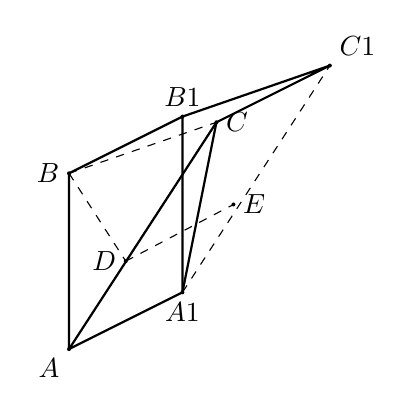
\begin{tikzpicture}[scale=.72,>=stealth]
\coordinate (A) at (0,0); \coordinate (B) at (0,3.1);
\coordinate (C) at (2.6,4.0); \coordinate (A1) at (2.0,1.0);
\coordinate (B1) at (2.0,4.1); \coordinate (C1) at (4.6,5.0);
\coordinate (D) at (1.0,1.55); \coordinate (E) at (2.9,2.55);
\draw[thick] (A)--(B)--(B1)--(A1)--cycle;
\draw[thick] (B1)--(C1)--(C)--(A);
\draw[dashed] (A)--(A1) (B)--(C) (A1)--(C1);
\draw[dashed] (D)--(E) (B)--(D)--(C);
\draw[thick] (A1)--(C);
\foreach \p/\pos in {A/below left,B/left,C/right,A1/below,B1/above,C1/above right,D/left,E/right}
  {\fill (\p) circle (1pt) node[\pos] {$\p$};}
\end{tikzpicture}
\end{center}
\nopagebreak[4]
（1） 证明：$AB=AC$；

（2） 设二面角 $A-BD-C$ 为 $60^\circ$，求 $B_1C$ 与平面 $BCD$ 所成的角的大小。

\end{question}
\begin{question}
\gkti{19}设数列 $\{a_n\}$ 的前 $n$ 项和为 $S_n$，已知 $a_1=1$，$S_{n+1}=4a_n+2$。

（1） 设 $b_n=a_{n+1}-2a_n$，证明数列 $\{b_n\}$ 是等比数列；

（2） 求数列 $\{a_n\}$ 的通项公式。

\end{question}
\begin{question}
\gkti{20}某车间甲组有 $10$ 名工人，其中有 $4$ 名女工人；乙组有 $5$ 名工人，其中有 $3$ 名女工人。现采用分层抽样方法（层内采用不放回简单随机抽样）从甲、乙两组中共抽取 $3$ 名工人进行技术考核。

（1） 求从甲、乙两组各抽取的人数；

（2） 求从甲组抽取的工人中恰有 $1$ 名女工人的概率；

（3） 记 $\xi$ 表示抽取的 $3$ 名工人中男工人数，求 $\xi$ 的分布列及数学期望。

\end{question}
\begin{question}
\gkti{21}已知椭圆 $C:\dfrac{x^2}{a^2}+\dfrac{y^2}{b^2}=1$（$a>b>0$）的离心率为 $\dfrac{\sqrt3}{3}$，过右焦点 $F$ 的直线 $l$ 与 $C$ 相交于 $A\text{、}B$ 两点，当 $l$ 的斜率为 $1$ 时，坐标原点 $O$ 到 $l$ 的距离为 $\dfrac{\sqrt2}{2}$。

（1） 求 $a\text{、}b$ 的值；

（2） $C$ 上是否存在点 $P$，使得当 $l$ 绕 $F$ 转到某一位置时，有 $\overrightarrow{OP}=\overrightarrow{OA}+\overrightarrow{OB}$ 成立？若存在，求出所有的 $P$ 的坐标与 $l$ 的方程；若不存在，说明理由。

\end{question}
\begin{question}
\gkti{22}设函数 $f(x)=x^2+a\ln(1+x)$ 有两个极值点 $x_1\text{、}x_2$，且 $x_1<x_2$。

（1） 求 $a$ 的取值范围，并讨论 $f(x)$ 的单调性；

（2） 证明：$f(x_2)>\dfrac{1-2\ln2}{4}$。

\end{question}